%% Based on a TeXnicCenter-Template by Gyorgy SZEIDL.
%%%%%%%%%%%%%%%%%%%%%%%%%%%%%%%%%%%%%%%%%%%%%%%%%%%%%%%%%%%%%

%----------------------------------------------------------
%
\documentclass{report}%
%
%----------------------------------------------------------
% This is a sample document for the standard LaTeX Report Class
% Class options
%       --  Body text point size:
%                        10pt (default), 11pt, 12pt
%       --  Paper size:  letterpaper (8.5x11 inch, default)
%                        a4paper, a5paper, b5paper,
%                       legalpaper, executivepaper
%       --  Orientation (portrait is the default):
%                       landscape
%       --  Printside:  oneside (default), twoside
%       --  Quality:    final (default), draft
%       --  Title page: titlepage, notitlepage
%       --  Columns:    onecolumn (default), twocolumn
%       --  Start chapter on left:
%                       openright(no), openany (default)
%       --  Equation numbering (equation numbers on right is the default)
%                       leqno
%       --  Displayed equations (centered is the default)
%                       fleqn (flush left)
%       --  Open bibliography style (closed bibliography is the default)
%                       openbib
% For instance the command
%          \documentclass[a4paper,12p,leqno]{report}
% ensures that the paper size is a4, fonts are typeset at the size 12p
% and the equation numbers are on the left side.
%
\usepackage{amsmath}%
\usepackage{amsfonts}%
\usepackage{amssymb}%
\usepackage{graphicx}
%----------------------------------------------------------
\usepackage{url}
\usepackage{tabularx}
%\usepackage{tablefootnote}
\usepackage[square,sort,comma,numbers]{natbib}
\usepackage{chapterbib}
\usepackage{hyperref}
\usepackage{url}
\usepackage{doi}
\usepackage{listings}
\usepackage{color}
%----------------------------------------------------------
% Define colors:
\definecolor{dkgreen}{rgb}{0,0.6,0}
\definecolor{gray}{rgb}{0.5,0.5,0.5}
\definecolor{mauve}{rgb}{0.58,0,0.82}
% Define language
\lstdefinelanguage{torxakis}
{
  % list of keywords
  morekeywords={
    PROCDEF,
    FUNCDEF
  },
  sensitive=false, % keywords are not case-sensitive
  morecomment=[l]{//}, % l is for line comment
  morecomment=[s]{/*}{*/}, % s is for start and end delimiter
  morestring=[b]" % defines that strings are enclosed in double quotes
}
% Define environment:
\lstset{frame=tb,
  language=torxakis,
  aboveskip=3mm,
  belowskip=3mm,
  showstringspaces=false,
  columns=flexible,
  basicstyle={\small\ttfamily},
  numbers=none,
  numberstyle=\tiny\color{gray},
  keywordstyle=\color{blue},
  commentstyle=\color{dkgreen},
  stringstyle=\color{mauve},
  breaklines=true,
  breakatwhitespace=true,
  tabsize=3
}
%----------------------------------------------------------
\usepackage{hyperref}

\usepackage{multicol}
\usepackage[shortlabels]{enumitem}

\usepackage{mathtools}
\usepackage[all,cmtip]{xy}

\usepackage{tabularx}
\def\tabularxcolumn#1{m{#1}}
\newcolumntype{Y}{>{\centering\arraybackslash}X}
%----------------------------------------------------------
\newcommand{\txs}{TorXakis}
\newcommand{\lpeq}{LPEQ}
\newcommand{\pedi}{Parallel / Enable / Disable / Interrupt}
\newcommand{\choice}{\texttt{\#\#} / Choice}
\newcommand{\txsChoice}[2]{#1\;\texttt{\#\#}\;#2}
\newcommand{\txsExit}{\texttt{EXIT}}
\newcommand{\txsEnable}[2]{#1\;\texttt{>>>}\;#2}
\newcommand{\txsDisable}[2]{#1\;\texttt{[>>}\;#2}
\newcommand{\txsInterrupt}[2]{#1\;\texttt{[><}\;#2}

\newcommand{\mcrl}{mCRL2}
\newcommand{\inlinecode}[1]{{\lstinline[language=torxakis]{#1}}}
\newcommand{\istep}{\texttt{ISTEP}}
\newcommand{\cistep}{\texttt{CISTEP}}
\newcommand{\true}{\textbf{true}}
\newcommand{\false}{\textbf{false}}
\newcommand{\comma}{,\;}
\newcommand{\labeledas}[1]{labeled as `#1'}
\newcommand{\labeledaseither}[2]{labeled as `#1' or `#2'}
\newcommand{\removelabelfrom}[1]{remove the label `#1' from}
\newcommand{\varsof}[1]{\text{vars}(#1)}
\newcommand{\sortof}[1]{\text{sort}(#1)}
\newcommand{\flsortof}[1]{\text{fl}(\sortof{#1})}

\newcommand{\primed}[1]{{#1}^\prime}
\newcommand{\pair}[2]{(#1\comma #2)}
\newcommand{\triple}[3]{(#1\comma #2\comma #3)}
\newcommand{\fourTuple}[4]{(#1\comma #2\comma #3\comma #4)}
\newcommand{\fiveTuple}[5]{(#1\comma #2\comma #3\comma #4\comma #5)}
\newcommand{\set}[1]{\{\;#1\;\}}
\newcommand{\setcomp}[2]{\{\;#1\;|\;#2\;\}}
\newcommand{\listcomp}[2]{[\;#1\;|\;#2\;]}
\newcommand{\qdot}{\; .\;}
\newcommand{\angleset}[1]{\langle\;#1\;\rangle}

\newcommand{\summandList}[1]{\textsc{smds}(#1)}
\newcommand{\starterSummands}[1]{\textsc{starters}(#1)}
\newcommand{\filteredStarterSummands}[2]{\textsc{starters}_{#1}(#2)}
\newcommand{\possibleSuccessors}[1]{\textsc{psuccs}(#1)}
\newcommand{\possiblePredecessors}[1]{\textsc{ppreds}(#1)}
\newcommand{\filteredPossibleSuccessors}[2]{\textsc{psuccs}_{#1}(#2)}
\newcommand{\nonDetSummands}[1]{\textsc{nondet}(#1)}
\newcommand{\enabledStarterSignature}[1]{\textsc{ESS}(#1)}
\newcommand{\enabledSuccessorSignature}[1]{\textsc{ESS}(#1)}
\newcommand{\nextESS}[1]{\textsc{next}(#1)}
\newcommand{\flattenESSs}[1]{\textsc{flatten}(#1)}
\newcommand{\dataParId}[2]{\textsc{pids}_#2(#1)}
\newcommand{\dataParIds}[0]{\textsc{pids}}
%----------------------------------------------------------
\setlength\parindent{0pt}
%----------------------------------------------------------
%\makeatletter
%\newcommand\footnoteref[1]{\protected@xdef\@thefnmark{\ref*{#1}}\@footnotemark}
%\makeatother
%----------------------------------------------------------
\newtheorem{theorem}{Theorem}
\newtheorem{acknowledgement}[theorem]{Acknowledgement}
\newtheorem{algorithm}[theorem]{Algorithm}
\newtheorem{axiom}[theorem]{Axiom}
\newtheorem{case}[theorem]{Case}
\newtheorem{claim}[theorem]{Claim}
\newtheorem{conclusion}[theorem]{Conclusion}
\newtheorem{condition}[theorem]{Condition}
\newtheorem{conjecture}[theorem]{Conjecture}
\newtheorem{corollary}[theorem]{Corollary}
\newtheorem{criterion}[theorem]{Criterion}
\newtheorem{definition}[theorem]{Definition}
\newtheorem{example}[theorem]{Example}
\newtheorem{exercise}[theorem]{Exercise}
\newtheorem{lemma}[theorem]{Lemma}
\newtheorem{notation}[theorem]{Notation}
\newtheorem{problem}[theorem]{Problem}
\newtheorem{proposition}[theorem]{Proposition}
\newtheorem{remark}[theorem]{Remark}
\newtheorem{solution}[theorem]{Solution}
\newtheorem{summary}[theorem]{Summary}
\newenvironment{proof}[1][Proof]{\textbf{#1.} }{\ \rule{0.5em}{0.5em}}
%----------------------------------------------------------
\begin{document}

\title{LPEQ\\\large{A linearization algorithm for \txs{}}}
\author{Djurre van der Wal}
\date{\today}
\maketitle
\tableofcontents

\chapter{Introduction}

Linearization gives a model a more regular structure.

Regular structure improves prospects of automated analysis and refactoring, which may in turn boost performance.

\lpeq{} is not intended to be fast/optimal.

\lpeq{} is developed as a more easily maintainable version of an existing implementation.


\chapter{Main algorithm}

\section*{Introduction}

\lpeq{} consists of 10 main phases:
\begin{enumerate}[1.]
\item Rewrite output values to input values.
\item Eliminate locally defined constants.
\item Eliminate of state automata (unsupported).
\item Create new processes for all sub-expressions of \pedi{} expressions, which are called `threads'; replace the sub-expressions themselves by instantiations of those processes.
\item Create new processes for each combination of channel parameters with which a process is instantiated (this is called `channel flattening').
\item Construct a process dependency tree from the model in order to confirm that the model does not contain parallel recursion.
\item Add a program counter to each process.
Associate all sequential expressions with a unique value of the program counter, and rewrite processes so that they become disjunctions of recursive process instantiations (typically in combination with an action prefix) and guarded \pedi{} expressions.
\item Rewrite processes so that all recursive process instantiations have an action prefix (this is called `prefix resolution').
\item Linearize \pedi{} expressions.
So far, this has only been developed for the Parallel expression.
\end{enumerate}

The phases can also be found in Figure~\ref{main-flow:fig}.

\begin{figure}[!ht]
\begin{center}
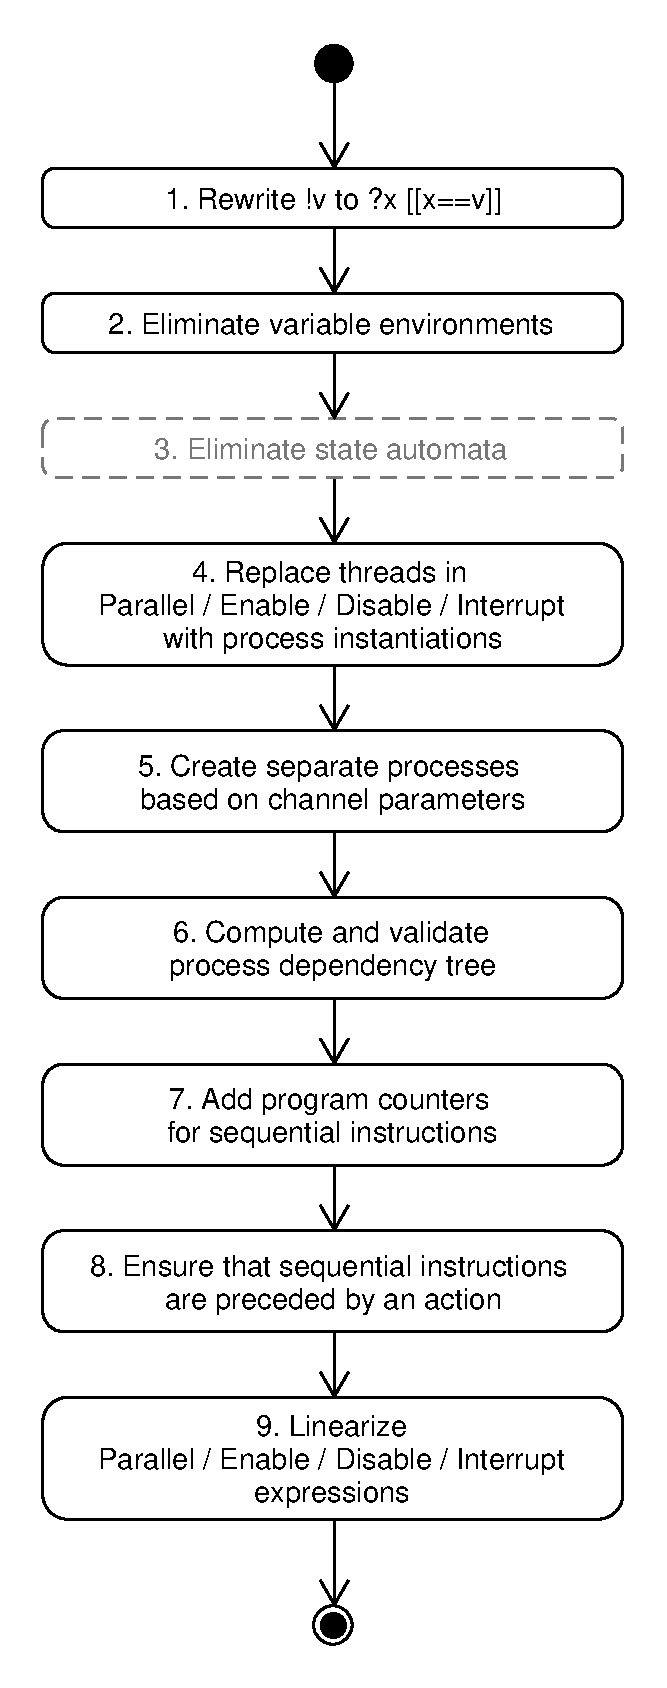
\includegraphics[width=0.5\linewidth]{umlet/linearization-main-flow}
\caption{Phases of the main algorithm.}
\label{main-flow:fig}
\end{center}
\end{figure}

\begin{samepage}
\section{Rewriting output values to input values}

\lpeq{} performs a depth-first search on the behavioral expression of the model.
When it encounters an action prefix $A$, it looks for all occurrences of the form $\texttt{!}v$ (where $v$ is an expression) in $A$.
For each occurrence, \lpeq{} does the following:
\begin{enumerate}[1.]
\item A fresh variable $x$ of the same sort as $v$ is introduced.
\item $\texttt{!}v$ is replaced by $\texttt{?}x$, the declaration of $x$.
\item $g_A$, the guard of $A$, is changed to $g_A \land x = v$.
\end{enumerate}
\end{samepage}

\section{Eliminating locally defined constants}

In the behavioral expressions of \txs{}, constants can be defined locally with a \texttt{LET} expression.
Such expressions are also called `variable environments'.

\lpeq{} eliminates \texttt{LET} expressions through substitution.

\section{Eliminating state-automaton expressions}

\lpeq{} cannot handle this yet.

\section{Instantiating threads} \label{thread-inst:section}

\pedi{} expressions include at least two sub-expressions.
Some of these sub-expressions are considered to run concurrently or may run concurrently `with themselves' in case of recursion.
These sub-expressions are therefore called `threads'.

Furthermore, we distinguish a subcategory of threads that are called `stackable'.
A \emph{stackable thread} is a thread of which there can exist multiple concurrent instances -- as a result of recursive instantiation -- but where only the most recently started instance can take actions.
(Note that the existence of stackable threads makes the state size automatically unbounded.)

Table~\ref{txsthreads:table} gives an overview of the threads that have been identified in the semantics of \txs{}.
The following subsections give more information about why certain sub-expressions have been categorized in the way that they are.

\begin{table}[!ht]
\begin{center}
\begin{tabularx}{\linewidth}{l|Y|Y|Y|Y|}
\textbf{Name} & \textbf{Expression} & \textbf{Stackable threads} & \textbf{Non-stackable threads} & \textbf{Other sub-expressions} \\ \hline
Parallel & $B_1 || \cdots || B_n$ & $\emptyset{}$ & $\set{B_1, \cdots{}, B_n}$ & $\emptyset{}$ \\ \hline
Enable & $\txsEnable{B_1}{B_2}$ & $\set{B_1}$ & $\emptyset{}$ & $\set{B_2}$ \\ \hline
Disable & $\txsDisable{B_1}{B_2}$ & $\emptyset{}$ & $\set{B_1}$ & $\set{B_2}$ \\ \hline
Interrupt & $\txsInterrupt{B_1}{B_2}$ & $\set{B_2}$ & $\set{B_1}$ & $\emptyset{}$ \\ \hline
\end{tabularx}
\caption{LPE rewrite operations.}
\label{txsthreads:table}
\end{center}
\end{table}

For convenience (and for the computation of the process dependency tree in phase 6, described in Section~\ref{procdeptree:section}) \lpeq{} does the following for each thread as well as for the root behavioral expression of the model:
\begin{enumerate}[1.]
\item A new process $P$ is created, with the thread expression as its body.
\item The sub-expression itself (at its original location) is replaced by the appropriate instantiation of $P$.
\end{enumerate}

(In the future, stackable and non-stackable threads can possibly be treated differently, thus increasing the range of linearizable models.)

\subsection{Enable threads}

Suppose that we have
\begin{align*}
P(x) = \txsEnable{(\txsChoice{a(x).P(x + 1)}{\txsExit{}})}{(b(x).\txsExit{})}
\end{align*}

This may result in a trace such as
\begin{align*}
a(1).a(2).a(3).\cdots{}.b(3).b(2).b(1)
\end{align*}

Informally, we observe that this behaviour can be simulated with a single process if we were to record the state of each instance of $P$ in a stack.
The left-hand side of Enable is therefore categorized as `stackable'.

The right-hand sub-expression \emph{can} contain recursion without causing issues, because all behaviour of the left-hand side of Enable `has already been popped' when the right-hand sub-expression is eventually executed.

\subsection{Disable threads}

Suppose that we have
\begin{align*}
P(x) = \txsDisable{(\txsChoice{a(x).P(x + 1)}{\txsExit{}})}{b(x)}
\end{align*}

This may result in traces such as
\begin{align*}
&a(1).a(2).a(3).\cdots{}.b(3).b(2).b(1) \\
&a(1).a(2).a(3).\cdots{}.b(2).b(1) \\
&a(1).a(2).a(3).\cdots{}.b(1) \\
&a(1).a(2).a(3).\cdots{}.b(3).b(1) \\
&a(1).a(2).a(3).\cdots{}.b(2) \\
&\cdots{}
\end{align*}

Informally, we observe that as a consequence of the recursion in the first sub-expression \txs{} is required to make a non-deterministic choice between an unbounded number of actions (all actions that originate from $b(x)$).
Unbounded quantification is not allowed in \txs{}, and we can only think of single-process implementations that would produce extra \istep{} actions that are not present in the input model. (In particular, the top element of a process stack could be popped non-deterministically.)

Unsurprisingly, we therefore consider the right-hand sub-expression of Enable to be a non-stackable thread.

Also consider the situation
\begin{align*}
P(x) = \txsDisable{(a(x).b(x).\txsExit{})}{(c(x).P(x + 1))}
\end{align*}

which may result in a trace such as
\begin{align*}
a(1).c(1).a(2).c(2).a(3).b(3)
\end{align*}

This example illustrates that there is no stacking behaviour when there is only recursion in the right-hand sub-expression of Disable.
The sub-expression is not a thread (or rather, it does not have to be treated as a thread).

\subsection{Interrupt threads}

Suppose that we have the situation
\begin{align*}
P(x) = \txsInterrupt{(\txsChoice{a(x).b(x).P(x + 1)}{\txsExit{}})}{(c(x).d(x).\txsExit{})}
\end{align*}

This may result in a trace such as
\begin{align*}
a(1).b(1).a(2).\textbf{c(2).c(1).d(1).d(2)}.b(2).a(3).\textbf{c(1).d(1)}.b(3)
\end{align*}

The number of expressions that can interrupt the left-hand sub-expression is unbounded, and \txs{} would have to choose between them non-deterministically.
\txs{} does not allow the quantification that this requires.
Consequently, the left-hand sub-expression is a non-stackable thread.

On the other hand, suppose that we have the situation
\begin{align*}
P(x) = \txsInterrupt{(a(x).b(x).\txsExit{})}{(c(x).P(x + 1))}
\end{align*}

This may result in traces such as
\begin{align*}
&a(1).c(1).a(2).b(2).b(1) \\
&a(1).b(1).c(1).a(2).c(2).a(3).c(3).a(4).b(4).b(3).b(2) \\
&\cdots{}
\end{align*}

We observe stack-like behaviour under these circumstances, which means that the right-hand sub-expression of Interrupt is a stackable thread.

\section{Flattening channels}

\txs{} processes refer to channels, but the actual channel instances that are used depend on the channel parameters that were used when they were instantiated.
To change this, \lpeq{} requires all combinations of actual channel instances with which processes are instantiated.

Consider a process instantiation $I$.
Within the context of this phase, the \emph{signature} of $I$ refers to the process that is instantiated by $I$ in combination with the actual channel instances that are passed as channel parameters (in order).

At the start of this phase, \lpeq{} performs a depth-first search for signatures on the behavioral expression of the model (this expression may have been changed by earlier phases).
\lpeq{} will only recurse into a process instantiation if it produced a new signature.

For each signature that was found, \lpeq{} does the following:
\begin{enumerate}[1.]
\item A new process $P$ is created, initially with the same body as the body of the process of the signature.
Instead of its original channel parameters \lpeq{} uses the actual channel instances of the model.
\item Each channel reference in $P$ is replaced by the corresponding actual channel instance from the signature.
\item Each process instantiation $I$ is replaced by an instantiation of the new process that corresponds with the signature of $I$.
\end{enumerate}

\lpeq{} only executes the third instruction after the first instruction has been executed for all signatures.

\section{Computing the process dependency tree} \label{procdeptree:section}

The \emph{process dependency tree} is a tree where each node has as a value a process $P$ and as branches the thread processes (see Section~\ref{thread-inst:section}) on which the \pedi{} expressions that occur in the body of $P$ depend.
The tree is computed by \lpeq{} with a straightforward depth-first search.

Note that a process dependency tree only contains thread processes: if a thread process can reach a \pedi{} expression by sequentially instantiating another process $P$ first, $P$ does not become a node of the tree.

The process dependency tree should be finite; otherwise, there may exist infinite parallel recursion in the model.
Infinite parallel recursion should be avoided because it may result in a situation where an action leads to infinitely many different states, violating one of the assumptions required for how \txs{} generates tests; and therefore \lpeq{} terminates with an error message when it detects that a process dependency tree is infinite.

\lpeq{} also takes the opportunity to check whether the model has no infinite sequential recursion: recursion where a process instantiates itself without doing an action prefix first.
Among other things, the absence of such recursion is a prerequisite for the termination of phase 8 (see Section~\ref{prefix-resolution:section}).

\section{Adding sequential program counters}

\subsection{Ensuring variable freshness}

In this phase, \lpeq{} will `merge' different processes.
These processes may use the same variables for different purposes.
To avoid conflicts in a lazy but foolproof manner, \lpeq{} first rewrites all involved processes so that each data parameter and each communication variable only occurs once (across processes).

\subsection{Updating process signatures}

Second, \lpeq{} does the following for each thread process (see Section~\ref{thread-inst:section}) $P$:
\begin{enumerate}[1.]
\item It gathers all variables that are (recursively) used by $P$.
This includes both data parameters and communication variables, but \emph{not} variables from thread processes on which $P$ depends.
\item It creates a fresh data parameter $\textit{pc}$ of sort \texttt{Int}.
This parameter can be interpreted as the \emph{program counter} of $P$.
\item It defines a new signature for $P$ (in particular, it defines new data parameters for $P$), consisting of $\textit{pc}$ and all variables gathered in the first instruction.
\lpeq{} also maintains a record of how process instantiations should be changed in accordance with the new signature.
\end{enumerate}

\subsection{Flattening sequential expressions} \label{flattenseqexprs:section}

Third, \lpeq{} recurses through the behavioral expression of each thread process $P$.
Meanwhile, simply put, the following work happens:
\begin{itemize}
\item A body of disjunctive behavioral expressions (a \choice{} expression) is composed, starting with zero expressions.
\lpeq{} will convert and add each behavioral sub-expression of $P$, recursing into regular processes (if not visited before) but not into other thread processes.
Each addition to the body has an appropriate program counter value associated with it, and they can be reached by instantiating $P$ with that value.
\item Instantiations of thread processes are updated (they require the initial value of the program counter, which is always \texttt{0}).
\item Instantiations of regular processes are changed to instantiations of $P$.
Each regular process is visited only once, and \lpeq{} maintains a record of the program counter value that is associated with visiting that process so that other visits can make use of the same value later.
\item Occurrences of \texttt{STOP} are replaced by an instantiation of $P$ in which the program counter is set to $\texttt{-1}$.
\end{itemize}

\lpeq{} does the above tasks for thread processes in such an order that when work starts on a thread process $P$ all thread processes on which $P$ depends have already been through the same procedure.
\lpeq{} extracts the order from the process dependency tree (see Section~\ref{procdeptree:section}): thread processes with a larger maximum distance to the root of the tree are processed \emph{before} thread processes with a smaller maximum distance to the root of the tree.

\section{Resolving prefixes} \label{prefix-resolution:section}

Where possible, \lpeq{} makes the structure of thread processes more regular by ensuring that recursive process instantiations are preceded by action prefixes (\pedi{} expressions are left alone again).
This is accomplished by substitution: \lpeq{} essentially repeatedly replaces recursive instantiations of a thread process $P$ without a preceding action prefix by the body of $P$ until a situation is reached where all instantiations of $P$ are preceded by action prefixes.
This procedure terminates because the model does not contain infinite sequential recursion, a property that is established in phase 6 (see Section~\ref{procdeptree:section}).

\clearpage
\section{Linearizing expressions with threads}

\subsection{Current state of the model}

By design, each thread process $P$ that is located on a leaf of the process dependency tree of the model in its current state is already (almost) linear: its body consists of a single \choice{} expression, and the choices consist of an action prefix followed by an instantiation of $P$, possibly nested in a \texttt{HIDE} expression.
Only the last part violates the requirements for linearity.

A thread process $Q$ that exists elsewhere in the process dependency tree is, of course, \emph{not} linear: even though its body consists of a single \choice{} expression, its choices can have two forms.
These forms are:
\begin{itemize}
\item An action prefix followed by an instantiation of $Q$, possibly nested in a \texttt{HIDE} expression (this form satisfies linearity except for the \texttt{HIDE} expression).
\item A guard followed by a \pedi{} expression, possibly nested in a \texttt{HIDE} expression.
It will take specific actions to linearize choices of this form, of which $Q$ contains at least one.
\end{itemize}

\subsection{General flow}

For each thread process $P$, \lpeq{} does the following:
\begin{enumerate}[1.]
\item It separates choices with a \pedi{} expression from choices without a \pedi{} expression.
\item Choices without a \pedi{} expression are used as the start of a fresh body of $P$.
\item One by one, choices with a \pedi{} expression are linearized.
In preparation, \lpeq{} rewrites the thread processes on which a \pedi{} expression depends so that they no longer contain \texttt{HIDE} expressions.
Linearization of the \pedi{} expression results in a number of new choices that are added to the new body of $P$ that is being composed.
\item \lpeq{} does another round of \emph{prefix resolution} (see Section~\ref{prefix-resolution:section}).
The reason for this simple, namely that some linearization methods produce choices that do not have an action prefix.
\end{enumerate}

\lpeq{} does the above tasks for thread processes in such an order that when work starts on a thread process $P$ all thread processes on which $P$ depends have already been through the same procedure.
\lpeq{} extracts the order from the process dependency tree (see Section~\ref{procdeptree:section}): thread processes with a larger maximum distance to the root of the tree are processed \emph{before} thread processes with a smaller maximum distance to the root of the tree.

A graphical overview of the procedure can also be found in Figure~\ref{pbranch-flow:fig}.

\begin{figure}[!ht]
\begin{center}
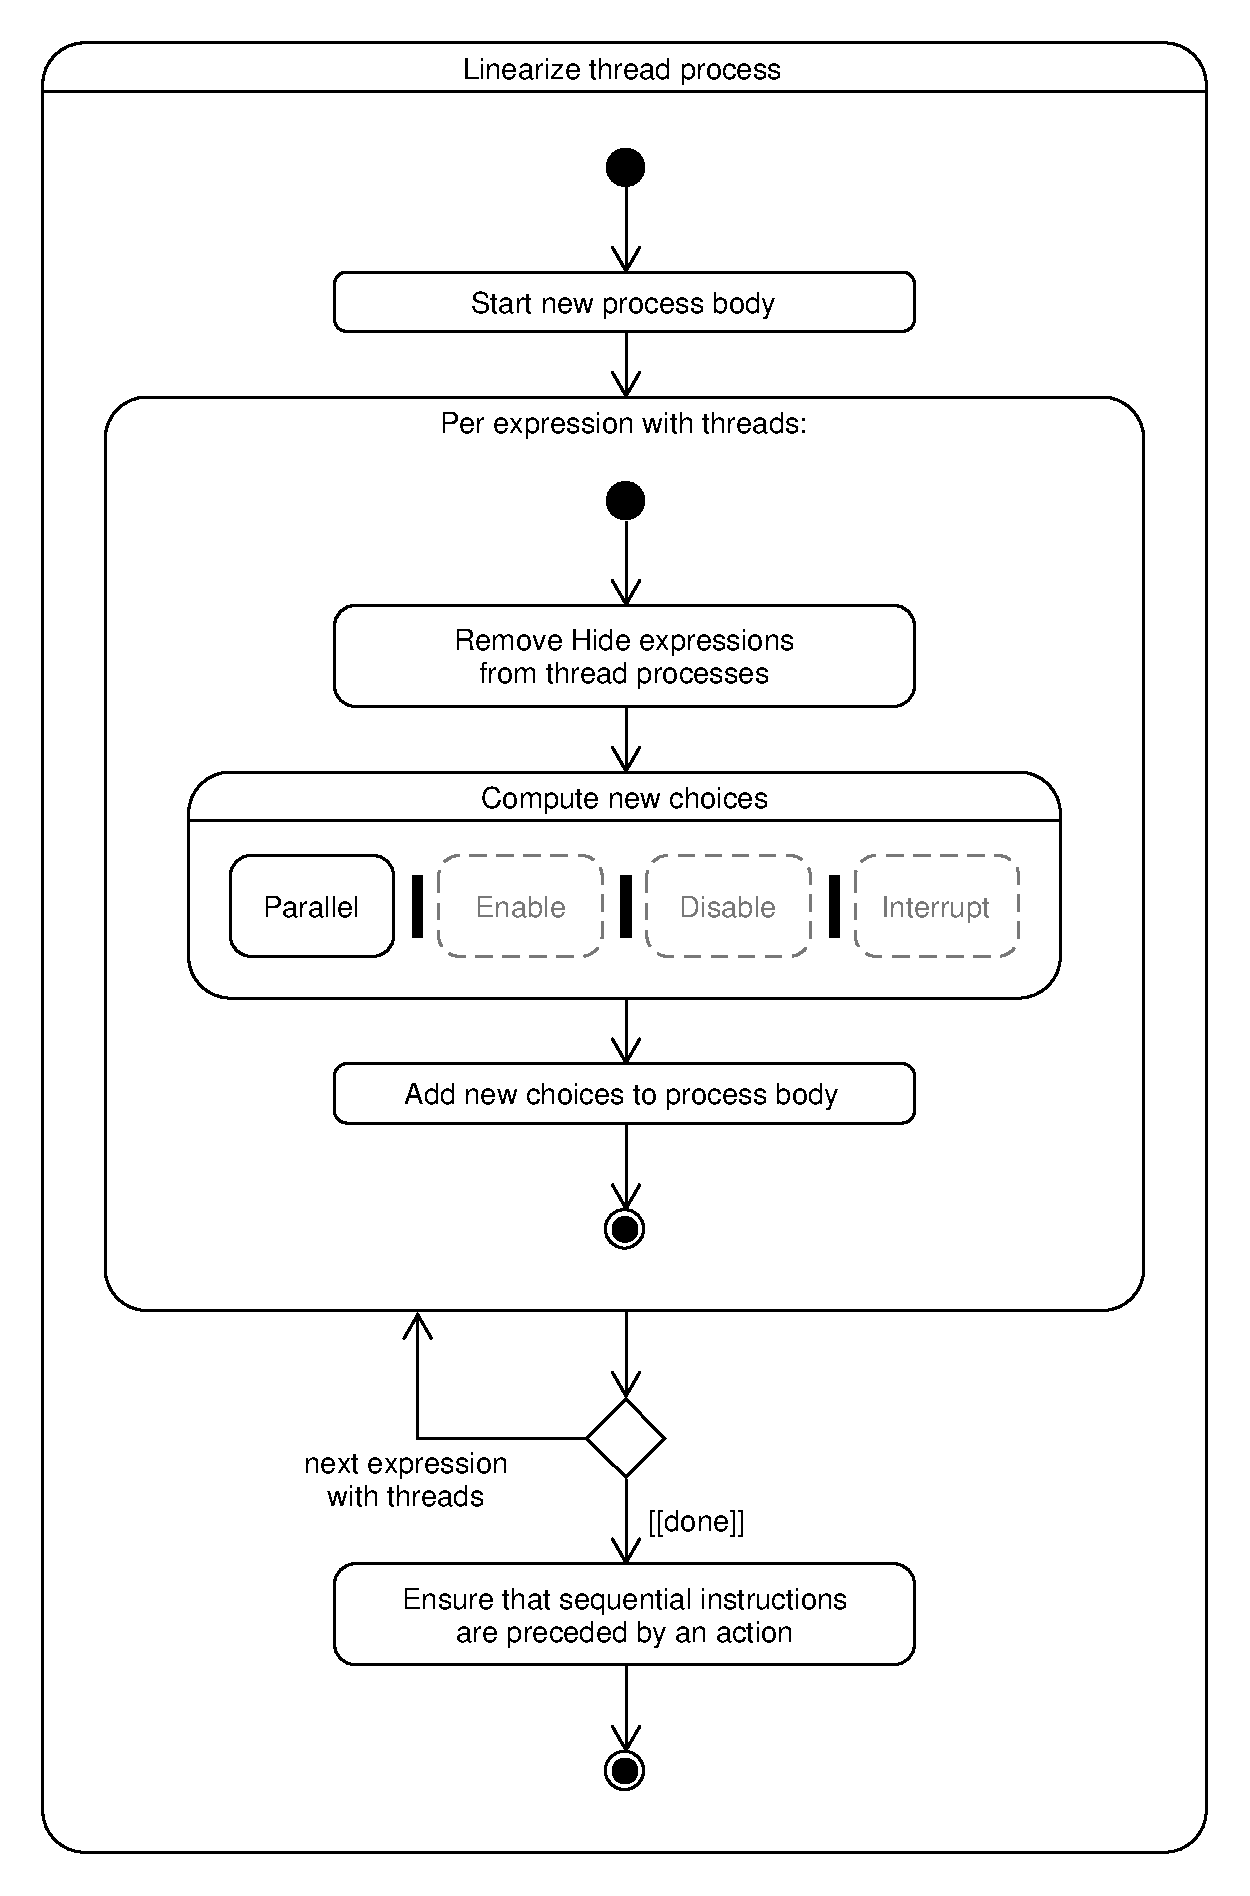
\includegraphics[width=0.8\linewidth]{umlet/linearization-pbranch-flow}
\caption{Flow for linearizing expressions with threads.}
\label{pbranch-flow:fig}
\end{center}
\end{figure}

\clearpage
\subsection{Eliminating HIDE expressions}

\lpeq{} eliminates \texttt{HIDE} expressions as follows:
\begin{enumerate}[1.]
\item \lpeq{} gathers all channels that are hidden by the \texttt{HIDE} expressions of a thread process $P$.
For each hidden channel $C$, it creates a new data parameter $f_C$ for $P$ of sort \texttt{Bool}.
$f_C$ can be interpreted as a flag that indicates whether $C$ is `currently' visible; in other words, $f_C$ is \texttt{True} if $C$ is visible, and $f_C$ is \texttt{False} if $C$ is hidden.
\item Then \lpeq{} rewrites all choices in the body of $P$ as follows.
If a choice has a \texttt{HIDE} expression, then the flags that correspond to the channels that are hidden by that \texttt{HIDE} expression are set to \texttt{False} in the process instantiation of that choice.
All other flags keep their original values.
The \texttt{HIDE} expression is removed.
\item The new choices in the body of $P$ are rewritten again for each channel $c$ for which there exists a flag $f_c$.
If the action prefix of a choice contains $c$, that choice is replaced by two new choices:
\begin{itemize}
\item One in which $f_c \texttt{ == True}$ has been added to the guard, and in which $c$ is still visible.
\item One in which $f_c \texttt{ == False}$ has been added to the guard, and in which $c$ has been removed (its parameter expressions become hidden parameter expressions).
In the process instantiation of the choice, $f_c$ is set to \texttt{False}.
\end{itemize}
Note that a choice is replaced by $2^n$ new choices if it contains $n$ channels that were hidden anywhere in the original thread process $P$!
\end{enumerate}

\subsection{Specific flows}

How \pedi{} expressions are linearized is described in the next Chapter~\ref{pbranch-flows:chapter}.


\chapter{Linearizing expressions with threads} \label{pbranch-flows:chapter}

\section{Linearizing Parallel}

Let $E$ be a Parallel expression that synchronizes the channels in the set $Z$ somewhere in a thread process $P$.

\subsection{Ensuring variable freshness}

Soon, \lpeq{} will be `merging' thread processes.
These processes may use the same variables for different purposes, or there may be multiple instances of the same variable (because a thread process is instantiated multiple times).

To avoid conflicts in a lazy but foolproof manner, \lpeq{} rewrites multiple threads of $E$ that depend on the same thread process $Q$ so that they each rely on a unique copy of $Q$ instead.
Then \lpeq{} rewrites all thread processes of $E$ so that each data parameter and each communication variable only occurs once (across processes).
All variables of all threads are now distinguishable and ready for the remainder of this procedure.

\subsection{Updating process signature}

\lpeq{} introduces a fresh data parameter $i_T$ for each thread $T$ of $E$.
\lpeq{} also gathers the data parameters of all thread processes on which $E$ depends (which are all unique).
Finally, \lpeq{} defines a new signature for $P$ (in particular, it defines new data parameters for $P$), consisting of $i_T$ for all $T$ of $E$ and all data parameters that were gathered.

\begin{samepage}
\subsection{Partitioning channels} \label{channelpartitions:subsection}

Let $C_E$ be the set of all multi-channels -- remember, an action prefix can contain multiple channels -- that occur across the threads of $E$.
The multi-channels are divided into two groups, $C_1$ and $C_2$, based on whether they share at least one channel with $Z$ or not, respectively.

$C_1$ and $C_2$ are used to process synchronizing actions and independent actions, respectively, which is described in the following sections.
\end{samepage}

\subsection{Processing synchronizing actions}

First, \lpeq{} `labels' all multi-channels in $C_1$ with their intersection with $Z$.
For example, multi-channels $\texttt{A|B}$ and $\texttt{A|C}$ can synchronize over $\texttt{A} \in Z$.
Simultaneously, multi-channels $\texttt{X|Y}$ and $\texttt{X|Z}$ might be able to synchronize over $\texttt{X} \in Z$.

For each unique label $L$ that has been encountered, \lpeq{} considers per thread all choices that have a multi-channel with label $L$.
\lpeq{} selects one considered choice per thread in all possible permutations.
(Note that if there is a thread where no choice has a multi-channel with label $L$, then there are zero permutations.)

Choice permutations in which multi-channels of different threads share channels that are \emph{not} in $Z$ are discarded.
This is a restriction on synchronization that can be found in the semantics of \txs{}.

Each remaining choice permutation $p$ is converted into $2^n$ new choices (where $n$ is the number of threads in $E$) because each thread could be initialized (indicated by $i_T \texttt{ == True}$) or uninitialized (indicated by $i_T \texttt{ == False}$).
For all possible different assumptions about this, a new choice $v$ is constructed:
\begin{itemize}
\item The guard of $v$ is a conjunction of the guards of all choices in $p$.
Furthermore, $i_T \texttt{ == True}$ or $i_T \texttt{ == False}$ is added to the guard for each $T$ in $E$ depending on whether $T$ is assumed to be initialized or not.
\item For each $c \in Z$, the communication variable of the channel offer of each choice in $p$ is replaced by a fresh variable of the same sort (all threads share the same fresh variables for the same channel $c$ and the same channel offer).
Appropriate substitutions are performed in the guard and in the recursive process instantiation.

After doing the above, the channel offers of all choices in $p$ are combined into one multi-channel.
\item In the recursive process instantiation of $v$, only the assignments from the choices in $p$ are used (all other data parameters remain unchanged).
Furthermore, for all $T$ in $E$, if the value of $i_T$ is \texttt{False}, we substitute the data parameters of the thread process of $T$ by the values that are used by the instantiation of that process.
\end{itemize}

\begin{samepage}
\subsection{Processing independent actions}

\lpeq{} considers all choices in all threads that have a multi-channel that occurs in $C_2$ (see Section~\ref{channelpartitions:subsection}).
According to the semantics of \txs{}, these choices can occur \emph{independently} of other threads.

For each choice $H$ belonging to a thread $T$, \lpeq{} creates two new choices:
\begin{itemize}
\item One in which $i_T \texttt{ == True}$ has been added to the guard.
In the recursive process instantiation, only the assignments from $H$ are used (all other data parameters remain unchanged).
\item One in which $i_T \texttt{ == False}$ has been added to the guard.
In the recursive process instantiation, only the assignments from $H$ are used (all other data parameters remain unchanged).
Since the value of $i_T$ means that the thread has not yet been initialized, we also substitute the data parameters of the thread process of $T$ by the values that are used by the instantiation of that process.
\end{itemize}
In both cases, the recursive process instantiation is also updated, of course ($i_T$ is set to \texttt{True}).
\end{samepage}

\section{Linearizing Enable}

Implemented and verified to work for some models, but undocumented.

\section{Linearizing Disable}

Implemented, but undocumented and untested.

\section{Linearizing Interrupt}

Implemented, but undocumented and untested.



\bibliographystyle{plainnat}
\bibliography{biblio}

\end{document}
